\documentclass[12pt,a4paper,oneside]{book}
\usepackage[utf8]{vietnam}
\usepackage{amsmath, amsthm, amssymb,latexsym,amscd,amsfonts,enumerate,titlesec,titletoc}
\usepackage[top=3.0cm, bottom=3.0cm, left=3.5cm, right=2.0cm]{geometry}
% căn lề theo quy chuẩn KLTN
\usepackage{color, fancyhdr, graphicx, wrapfig}
\usepackage[unicode]{hyperref}
\usepackage{indentfirst}
\usepackage{graphicx}
\usepackage{tikz}
\usepackage{array}
\usetikzlibrary{calc}
%\newtheorem{example}{Ví dụ}[section]
\def\chaptertitlename{\fontsize{14pt}{14pt}\selectfont{CHƯƠNG}}
\titleformat{\chapter}[display]
{\vspace{-2cm}\normalfont\Large\filcenter\bfseries}
{{{\chaptertitlename\,}\thechapter}} {0pc}{{}\MakeUppercase}
\theoremstyle{theorem}
\newtheorem{theorem}{Định lý}[section]
\theoremstyle{definition}
\newtheorem{theorem2}{Định nghĩa}[section]
\newtheorem{dn}[theorem2]{Định nghĩa}
\newtheorem{nx}[theorem2]{Nhận xét}
\newtheorem{vd}[theorem2]{Ví dụ}
\newtheorem{md}[theorem2]{Mệnh đề}
\newtheorem{tc}[theorem2]{Tính chất}
\newtheorem{bd}[theorem2]{Bổ đề} 
\newtheorem{dl}[theorem2]{Định lý}
\newtheorem{bt}[theorem2]{Bài toán}
\newtheorem{hq}[theorem2]{Hệ quả}
\newtheorem{cy}[theorem2]{Chú ý}
\newtheorem{ly}[theorem2]{Lưu ý}
\newtheorem{kn}[theorem2]{Khái niệm}
%\newtheorem{example}{Ví dụ}[section]
%\newtheorem{proposition}{Mệnh đề}[section]
%\newtheorem{definition}[proposition]{Định nghĩa}
%\newtheorem{remark}[proposition]{Nhận xét}
%\newtheorem{theorem}[proposition]{Định lý}
%\newtheorem{example}[proposition]{Ví dụ}
%\newtheorem{corollary}[proposition]{Hệ quả}
%\newtheorem{lemma}[proposition]{Bổ đề}
\newtheorem{Theorem}{Theorem}[section]
\newtheorem{Proposition}[Theorem]{Proposition}
\newtheorem{Remark}[Theorem]{Remark}
\newtheorem{Lemma}[Theorem]{Lemma}
\newtheorem{Corollary}[Theorem]{Corollary}
\newtheorem{Definition}[Theorem]{Definition}
\newtheorem{Example}[Theorem]{Example}
\newcommand{\br}[1]{\left(#1\right)} %ngoặc tròn
\newcommand{\brb}[1]{\left\{#1\right\}} %ngoặc nhọn, tập hợp
\newcommand{\brc}[1]{\left[#1\right]} %ngoặc vuông
\newcommand{\bao}[1]{\left<#1\right>} 
\newcommand{\tri}[1]{\left|#1\right|}
\newcommand{\flo}[1]{ \left \lfloor #1 \right \rfloor}
\newtheorem*{case1}{Trường hợp 1}
\newtheorem*{case2}{Trường hợp 2}
\newtheorem*{case3}{Trường hợp 3}
\newcommand{\aut}[1]{\mbox{Aut}\br{#1}}
\newcommand{\gal}[1]{\mbox{Gal}\br{#1}}
\newcommand{\Q}{\mathbb{Q}}
\newcommand{\Z}{\mathbb{Z}}



\renewcommand{\theequation}{\thesection.\arabic{equation}}
\normalsize
\pagestyle{fancy}
\makeatletter
\renewcommand{\ps@plain}{
	\renewcommand{\@oddfoot}{\textrm{\centerline{\thepage}}}
	\renewcommand{\@evenfoot}{\@oddfoot}
	\renewcommand{\@oddhead}{}
	\renewcommand{\@evenhead}{\@oddhead}}
\pagestyle{plain}

%%%%%%%%%%%%%%%%%
\begin{document}
	\fontsize{13pt}{18pt}\selectfont % Lệnh thay đổi cỡ chữ thành cỡ 14, cỡ dòng 18 (theo quy chuẩn của Khóa Luận TN).
	\setlength{\baselineskip}{26truept}
	%\fontsize{13pt}{14pt}\selectfont
	\pagenumbering{arabic}
	%\pagenumbering{roman}
	%\frontmatter
	\pagestyle{empty}
	\begin{titlepage}
		
\begin{tikzpicture}[remember picture,overlay,inner sep=0,outer sep=0]
			\draw[black,line width=3pt] ([xshift=-1.5cm,yshift=-2cm]current page.north east) coordinate (A)--([xshift=2.5cm,yshift=-2cm]current page.north west) coordinate(B)--([xshift=2.5cm,yshift=2cm]current page.south west) coordinate (C)--([xshift=-1.5cm,yshift=2cm]current page.south east) coordinate(D)--cycle;
			
			\draw[black,line width=1pt] ([xshift=-1.7cm,yshift=-2.2cm]current page.north east) coordinate (A)--([xshift=2.7cm,yshift=-2.2cm]current page.north west) coordinate(B)--([xshift=2.7cm,yshift=2.2cm]current page.south west) coordinate (C)--([xshift=-1.7cm,yshift=2.2cm]current page.south east) coordinate(D)--cycle;
			
		\end{tikzpicture}
		\begin{center}
			\vspace{-1cm}\textbf{TRƯỜNG ĐẠI HỌC SƯ PHẠM, ĐẠI HỌC HUẾ}
			
			\vspace{7pt}
			\bf\underline{KHOA TOÁN HỌC}
		\end{center}
		\vspace{10pt}
        \begin{center}
        
\includegraphics[width=0.4\textwidth]{Hinh.jpg}
        \end{center}
		\begin{center}
			
			\vspace{2cm}
			\fontsize{13pt}{13pt}\selectfont 
			\textbf{TIỂU LUẬN TÍCH HỢP CÔNG NGHỆ THÔNG TIN TRONG DẠY HỌC TOÁN} 
			
			\vspace{10pt}
			
		\end{center}
		\vspace{1cm}
		\begin{center}
			\fontsize{18pt}{17pt}\selectfont 
			\bf\fontsize{15pt}{19}\selectfont ĐỒ THỊ HÀM SỐ\\TRONG CÁC TÌNH HUỐNG THỰC TẾ
		\end{center}	
		
		\vspace{1.5cm}
		\hspace{-0.6cm}\begin{tabular}{cc}{\fontsize{13pt}{16}\selectfont Giảng viên hướng dẫn}&\hspace{1cm}{\fontsize{12pt}{16}\selectfont Sinh viên thực hiện}\\
			\hspace{-0.6cm}\bf\fontsize{13pt}{16}\selectfont TS NGUYỄN ĐĂNG MINH PHÚC&\hspace{1cm}{\bf\fontsize{12pt}{16}\selectfont NGUYỄN THỊ THANH HÀ}\\ 
			&\hspace{1cm}{\bf\fontsize{13pt}{16}\selectfont MSSV: 23S1010008}
		\end{tabular}
		\vfill
		\centerline {\bf Huế, 09/2026}
	\end{titlepage}
	
	%%%%%%%%%%%%%%%%%%%%%%%%%%%%%%%%%%%%%%%%%%%%%%%%%%%%%%%%%%
	
	\fontsize{13pt}{18pt}\selectfont % Lệnh thay đổi cỡ chữ thành cỡ 14, cỡ dòng 18 (theo quy chuẩn của Khóa Luận TN).
	\setlength{\baselineskip}{26truept}
	%\fontsize{13pt}{14pt}\selectfont
	\pagenumbering{arabic}
	%\pagenumbering{roman}
	%\frontmatter
	\pagestyle{empty}
	
    \chapter{KIẾN THỨC CHUẨN BỊ}
    Chương này tổng hợp và hệ thống hóa các kiến thức nền tảng về hàm số và đồ thị hàm số, bao gồm tính đơn điệu, cực trị, giá trị lớn nhất – giá trị nhỏ nhất, đường tiệm cận và quy trình khảo sát đồ thị. Đây là cơ sở lý thuyết quan trọng làm nền tảng cho việc phân tích và giải quyết các bài toán thực tế ở Chương 2.
    \section{Nền tảng về tính đơn điệu và cực trị của hàm số}

    \noindent Cho $K \in \mathbb{R}$, trong đó $K$ là một khoảng, đoạn hoặc nửa khoảng.
    \subsection{Tính đơn điệu của hàm số}
        \begin{center}
        
\includegraphics[width=0.6\textwidth]{Hinh1.png}
        \end{center}
        \begin{dl}
            Cho hàm số $y=f(x)$ có đạo hàm trên tập $K$. Nếu $f'(x) \geq 0$ hoặc $f'(x) \leq 0$ với mọi $x$ thuộc $K$ và $f'(x)=0$ chỉ tại một số hữu hạn điểm của $K$ thì hàm số $f(x)$ đồng biến (hoặc nghịch biến) trên $K$.
        \end{dl}
    \subsection{Điểm cực trị, giá trị cực trị của hàm số}
        \begin{dn}
            Cho hàm số $y=f(x)$ xác định và liên tục trên khoảng $(a;b)$ ($a$ có thể là $- \infty$, $b$ có thể là $+ \infty$) và điểm $x_0 \in (a;b)$.
        \end{dn}
        \begin{itemize}
            \item[(i)] Nếu tồn tại số $h>0$ sao cho $f(x)<f(x_0)$ với mọi $x \in (x_0-h;x_0+h) \subset (a;b)$ và $x$ khác $x_0$ thì ta nói hàm số $f(x)$ đạt cực đại tại $x_0$.
            \item[(ii)] Nếu tồn tại số $h>0$ sao cho $f(x)>f(x_0)$ với mọi $x \in (x_0-h;x_0+h) \subset (a;b)$ và $x$ khác $x_0$ thì ta nói hàm số $f(x)$ đạt cực tiểu tại $x_0$.
        \end{itemize}
        \begin{cy}
            Nếu $x_0$ là một điểm cực trị của hàm số $y=f(x)$ thì điểm $M(x_0;f(x_0))$ được gọi là điểm cực trị của hàm số $y=f(x)$.
        \end{cy}
        \begin{dl}
            Giả sử hàm số $y=f(x)$ liên tục trên khoảng $(a;b)$ chứa điểm $x_0$ và có đạo hàm trên các khoảng $(a;x_0)$ và $(x_0;b)$. Khi đó
        \end{dl}
        \begin{itemize}
            \item[(i)] Nếu $f'(x)<0$ với mọi $x \in (a;x_0)$ và $f'(x)>0$ với mọi $x \in (x_0;b)$ thì $x_0$ là một điểm cực tiểu của hàm số $f(x)$.
            \item[(ii)] Nếu $f'(x)>0$ với mọi $x \in (a;x_0)$ và $f'(x)<0$ với mọi $x \in (x_0;b)$ thì $x_0$ là một điểm cực đại của hàm số $f(x)$.
        \end{itemize}  
    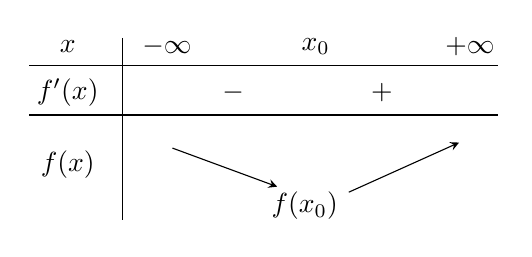
\begin{tikzpicture}[scale=0.7, >=stealth]
        % Các đường kẻ
        \draw (-1.5,0) -- (7,0);
        \draw (-1.5,-0.9) -- (7,-0.9);
        \draw (0.2,0.5) -- (0.2,-2.8);
        % Hàng x
        \node at (-0.8,0.35) {$x$};
        \node at (1,0.35) {$-\infty$};
        \node at (3.7,0.35) {$x_0$};
        \node at (6.5,0.35) {$+\infty$};
        % Hàng f'(x)
        \node at (-0.8,-0.5) {$f'(x)$};
        \node at (2.2,-0.5) {$-$};
        \node at (4.9,-0.5) {$+$};
        % Hàng f(x)
        \node at (-0.8,-1.8) {$f(x)$};
        % Mũi tên biến thiên
        \draw[->] (1.1,-1.5) -- (3.0,-2.2);
        \draw[->] (4.3,-2.3) -- (6.3,-1.4);
        % Giá trị cực tiểu
        \node at (3.5,-2.55) {$f(x_0)$};        
    \end{tikzpicture}  
    \hspace{1.5cm}
    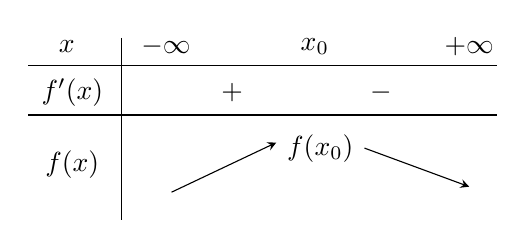
\begin{tikzpicture}[scale=0.7, >=stealth]        
        % Các đường kẻ
        \draw (8.5,0) -- (17,0);
        \draw (8.5,-0.9) -- (17,-0.9);
        \draw (10.2,0.5) -- (10.2,-2.8);        
        % Hàng x
        \node at (9.2,0.35) {$x$};
        \node at (11,0.35) {$-\infty$};
        \node at (13.7,0.35) {$x_0$};
        \node at (16.5,0.35) {$+\infty$};        
        % Hàng f'(x)
        \node at (9.3,-0.5) {$f'(x)$};
        \node at (12.2,-0.5) {$+$};
        \node at (14.9,-0.5) {$-$};        
        % Hàng f(x)
        \node at (9.3,-1.8) {$f(x)$};        
        % Mũi tên biến thiên
        \draw[->] (11.1,-2.3) -- (13.0,-1.4);
        \draw[->] (14.6,-1.5) -- (16.5,-2.2);        
        % Giá trị cực tiểu
        \node at (13.8,-1.5) {$f(x_0)$};       
    \end{tikzpicture}
    \subsection{Hàm đặc trưng}
        \begin{tc}
             Cho hàm số $y=f(x)$ đồng biến (hoặc nghịch biến) trên $K$. Khi đó với mọi $x \in K$:
             $$f(x_1)=f(x_2) \Leftrightarrow x_1=x_2; \quad f(x_1)>f(x_2) \Leftrightarrow x_1>x_2$$ 
        \end{tc}
        \begin{cy}
            Từ đó, trong nhiều bài toán, ta đưa phương trình về dạng $f(g(x)) = f(h(x))$ và biện luận nếu hàm $f(x)$ đơn điệu trên $K$ và $g(x), h(x)$ đều nhận giá trị trên $K$ thì phương trình $f(g(x)) = f(h(x)) \Leftrightarrow g(x) = h(x)$.
            \begin{itemize}
                \item[(i)] Nếu $f(x)$ đồng biến trên $K$ thì $f(g(x)) > f(h(x)) \Leftrightarrow g(x) > h(x)$.
                \item[(ii)] Nếu $f(x)$ nghịch biến trên $K$ thì $f(g(x)) < f(h(x)) \Leftrightarrow g(x) > h(x)$.
            \end{itemize}
        \end{cy}
        \begin{vd}
            Một phàn lát cắt của dãy núi có độ cao tính bằng mét được mô tả bởi hàm số
            $$y=h(x)=- \frac{1}{1320000}x^3+ \frac{9}{3520}x^2- \frac{81}{44}x+840 \text{ với } 0 \leq x \leq 2000$$
        \end{vd}
        \begin{center}
        
\includegraphics[width=0.9\textwidth]{Hinh2.png}
        \end{center}
        Tìm tọa độ các đỉnh của lát cắt dãy núi trên đoạn $[0;2000]$.
       
        Hướng dẫn giải:
        
        Ta có:
        $$h'(x)=- \frac{x^2}{440000}+ \frac{9x}{1760}- \frac{81}{44} \forall x \in (0;2000)$$

        Do đó $h'(x)=0 \Leftrightarrow 
            \left[
            \small \begin{aligned}
            x &= 450\\
            x &= 1800
            \end{aligned} 
            \right.
        $.
        Xét $h(450)=660,313$ và $h(1800)= \frac{15315}{11}$. 

        Do đó tọa độ các đỉnh của lát cắt dãy núi trên đoạn $[0;2000]$ là $(450;460,313)$ và $(1800; \dfrac{15315}{11})$.
    \section{Nền tảng về giá trị lớn nhất và giá trị nhỏ nhất của hàm số}
    \subsection{Định nghĩa}
        \begin{dn}
        Cho hàm số $f(x)$ xác định trên $D$.
        \end{dn}
        \begin{itemize}
            \item[(i)] Số $M$ được gọi là giá trị lớn nhất của hàm số $y=f(x)$ trên $D$, kí hiệu $M=max_Df(x)$ nếu
                \[
                \small \begin{cases}
                f(x) \leq M \forall x \in D\\
                \exists x_0 \in D| f(x_0)=M
                \end{cases}
                \]
            \item[(ii)] Số $m$ được gọi là giá trị nhỏ nhất của hàm số $y=f(x)$ trên $D$, kí hiệu $M=min_Df(x)$ nếu
                \[
                \small \begin{cases}
                f(x) \geq m \forall x \in D\\
                \exists x_0 \in D| f(x_0)=m
                \end{cases}
                \]
        \end{itemize}
    \subsection{Tìm giá trị lớn nhất và giá trị nhỏ nhất của hàm số liên tục}
        \begin{cy}
            Mọi hàm số liên tục trên một đoạn đều có giá trị lớn nhất và giá trị nhỏ nhất trên đoạn đó.
        \end{cy}
        Giả sử hàm số $f(x)$ liên tục trên đoạn $[a;b]$ và có đạo hàm trên khoảng $(a;b)$, có thể trừ đi một số hữu hạn điểm. Nếu $f'(x)=0$ chỉ tại một số hữu hạn điểm thuộc khoảng $(a;b)$ thì t có quy tắc tìm giá trị lớn nhất và giá trị nhỏ nhất của hàm số $f(x)$ trên đoạn $[a;b]$ như sau:
        \begin{itemize}
            \item[] \textit{Bước 1}. Tìm các điểm $x_1,x_2,...,x_n$ thuộc khoảng $(a;b)$ mà tại đó hàm số có đạo hàm bằng $0$ hoặc không tồn tại.
            \item[] \textit{Bước 2}. Tính $f(x_1),f(x_2),...,f(x_n),f(a) \text{ và } f(b)$.
            \item[] \textit{Bước 3}. So sánh các giá trị tìm được ở \textit{Bước 2}.
            \begin{nx}
                Số lớn nhất trong các giá trị đó là giá trị lớn nhát của hàm số $f(x)$ trên đoạn [a;b], số nhỏ nhát trong các giá trị đó là giá trị nhỏ nhất của hàm số $f(x)$ trên đoạn $[a;b]$.
            \end{nx}
        \end{itemize}
    \subsection{Lưu ý}
        \begin{itemize}
            \item[(i)] Lưu ý về giá trị lớn nhất và nhỏ nhất của hàm số $f(x)=asinx+bcosx$.\\
            Cho hàm số $f(x)=asinx+bcosx(a^2+b^2>0)$. Khi đó:
            $$maxf(x)= \sqrt{a^2+b^2};min f(x)=-\sqrt{a^2+b^2}$$
            \begin{hq}
                $max(asinx)= \lvert a \rvert; min(asinx)=-\lvert a \rvert$.
            \end{hq}
            \item[(ii)] Lưu ý về giá trị lớn nhất và giá trị nhỏ nhất của hàm số $f(u(x))$ trên $D$.\\
            Đặt $t=u(x)$, với $x \in D$, giả sử ta tìm được tập giá trị của $u(x)$ trên $D$ là $K$. Khi đó:
            $$max_{x\in D} f(u(x))= max_{i \in K} f(t)$$
            \item[(iii)] Bất đẳng thức Cauchy (BĐT AM-GM) cho 2 số và cho 3 số\\
            Cho $a,b$ là các số thực không âm, khi đó:
            $$\frac{a+b}{2} \geq \sqrt{ab}$$.
            Cho $a,b,c$ là các số thực không âm, khi đó:
            $$\frac{a+b+c}{3} \geq \sqrt[3]{abc}$$.
            \begin{hq}
                $ab \leq (\frac{a+b}{2})^2,abc \leq (\frac{a+b+c}{3})^3$ với $a,b,c \geq0$.
            \end{hq}
        \end{itemize}
        \begin{minipage}{0.68\textwidth}
        \begin{vd}
            Một miếng bìa hình tam giác đều $ABC$ có cạnh bằng $16$. Học sinh cắt một hình chữ nhật $MNPQ$ từ miếng bìa trên làm biển trông xe cho lớ học buổi ngoại khóa (với $M,N$ thuộc cạnh $BC$ và $P,Q$ lần lượt thuộc cạnh $AC$ và $AB$). Gọi $S$ là giá trị lớn nhất của diện tích hình chữ nhật $MNPQ$. Khi đó, giá trị $S^2$ bằng bao nhiêu?
        \end{vd}
        \end{minipage}
        \hfill
        \begin{minipage}{0.27\textwidth}
        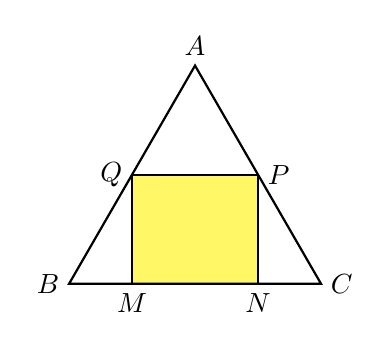
\begin{tikzpicture}[scale=0.4]
            % Các đỉnh tam giác
            \coordinate (A) at (4,6.928);
            \coordinate (B) at (0,0);
            \coordinate (C) at (8,0);
            % Các điểm
            \coordinate (M) at (2,0);
            \coordinate (N) at (6,0);
            \coordinate (Q) at (2,3.464);
            \coordinate (P) at (6,3.464);    
            % Tô hình chữ nhật
            \fill[yellow!60] (M) -- (N) -- (P) -- (Q) -- cycle;    
            % Tam giác
            \draw[thick] (A) -- (B) -- (C) -- cycle;
            % Hình chữ nhật
            \draw[thick] (M) -- (N) -- (P) -- (Q) -- cycle;
            % Nhãn
            \node[above] at (A) {$A$};
            \node[left] at (B) {$B$};
            \node[right] at (C) {$C$};
            \node[below] at (M) {$M$};
            \node[below] at (N) {$N$};
            \node[right] at (P) {$P$};
            \node[left] at (Q) {$Q$};
        \end{tikzpicture}
        \end{minipage}

        Hướng dẫn giải:
        
        Gọi $H$ là trung điểm của $BC$. Kẻ $AH$ cắt $PQ$ tại $K$.

         Đặt $PK=x$. Ta có $PQ=2x\;(0<x<8)$.
        \begin{center}
        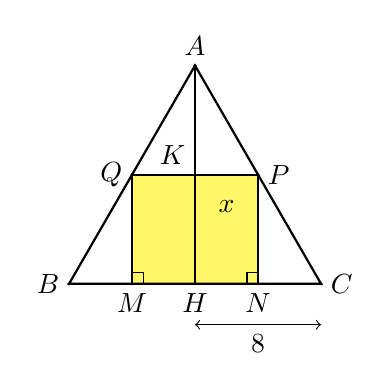
\begin{tikzpicture}[scale=0.4]
            % Các đỉnh tam giác
            \coordinate (A) at (4,6.928);
            \coordinate (B) at (0,0);
            \coordinate (C) at (8,0);
            % Các điểm
            \coordinate (M) at (2,0);
            \coordinate (N) at (6,0);
            \coordinate (H) at (4,0);
            \coordinate (Q) at (2,3.464);
            \coordinate (K) at (4,3.464);
            \coordinate (P) at (6,3.464);
            % Tô hình chữ nhật
            \fill[yellow!60] (M) -- (N) -- (P) -- (Q) -- cycle;
            % Tam giác ABC
            \draw[thick] (A) -- (B) -- (C) -- cycle;
            % Đường AH
            \draw[thick] (A) -- (H);
            % Hình chữ nhật MNPQ
            \draw[thick] (M) -- (N) -- (P) -- (Q) -- cycle;
            % Hai cạnh QM và PN
            \draw[thick] (Q) -- (M);
            \draw[thick] (P) -- (N);
            % Các điểm
            \fill (A) circle (1.5pt);
            \fill (B) circle (1.5pt);
            \fill (C) circle (1.5pt);
            \fill (M) circle (1.5pt);
            \fill (N) circle (1.5pt);
            \fill (H) circle (1.5pt);
            \fill (Q) circle (1.5pt);
            \fill (K) circle (1.5pt);
            \fill (P) circle (1.5pt);
            % Nhãn
            \node[above] at (A) {$A$};
            \node[left] at (B) {$B$};
            \node[right] at (C) {$C$};
            \node[below] at (M) {$M$};
            \node[below] at (N) {$N$};
            \node[below] at (H) {$H$};
            \node[left] at (Q) {$Q$};
            \node[above left] at (K) {$K$};
            \node[right] at (P) {$P$};
            % Đánh dấu x = KP
            \node at (5.0,2.45) {$x$};
            % Đánh dấu góc vuông tại M
            \draw (2,0.35) -- (2.35,0.35) -- (2.35,0);
            % Đánh dấu góc vuông tại N
            \draw (5.65,0) -- (5.65,0.35) -- (6,0.35);
            % Độ dài HC = 8
            \draw[<->] (4,-1.3) -- (8,-1.3);
            \node[below] at (6,-1.3) {$8$};
        \end{tikzpicture}
        \end{center}
        
        Có $PN \mathrel{/\!/} AH$ nên
        $
        \dfrac{PN}{AH}=\dfrac{CN}{CH}
        \Rightarrow \dfrac{PN}{\dfrac{\sqrt{3}}{2}BC}
        =\dfrac{8-x}{8} \Rightarrow  PN=\sqrt{3}(8-x).
        $
        
        Do đó $
        S_{MNPQ}
        =PQ.PN
        =2x\sqrt{3}(8-x)
        =2\sqrt{3}x(8-x)
        \leq
        2\sqrt{3}
        \left(\dfrac{x+8-x}{2}\right)^2.
        $
        
        (áp dụng $
        ab\leq\left(\dfrac{a+b}{2}\right)^2
        \forall a,b\in\mathbb{R}
        $).
        
        Vậy $S^2\leq(32\sqrt{3})^2=3072.$   
    \section{Tiệm cận của đồ thị hàm số}
    \subsection{Đường tiệm cận ngang}
        \begin{dn}
            Đường thẳng $y=y_0$ được gọi là \textit{đường tiệm cận ngang} của đồ thị hàm số $y=f(x)$ nếu:
            $$\lim_{x \to +\infty}f(x)=y_0 \text{ hoặc } \lim_{x \to -\infty}f(x)=y_0$$
        \end{dn}
        \begin{center}
        
\includegraphics[width=0.9\textwidth]{Hinh3.jpeg}
        \end{center}
    \subsection{Đường tiệm cận đứng}
        \begin{minipage}{0.63\textwidth}
        \begin{dn}
            Đường thẳng $x=x_0$ được gọi là \textit{đường tiệm cận đứng} của đồ thị hàm số $y=f(x)$ nếu ít nhất một trong các điều kiện sau được thỏa mãn:
             $$\lim_{x \to x_0^-}f(x)= +\infty;\quad lim_{x \to x_0^-}f(x)= -\infty;$$
             $$\lim_{x \to x_0^+}f(x)= +\infty;\quad lim_{x \to x_0^+}f(x)= -\infty.$$
        \end{dn}
        \end{minipage}
        \hfill
        \begin{minipage}{0.3\textwidth}
        
\includegraphics[width=0.9\textwidth]{Hinh4.png}
        \end{minipage}
    \subsection{Đường tiệm cận xiên}
        \begin{minipage}{0.63\textwidth}
        \begin{dn}
            Đường thẳng $y=ax+b(a \neq 0)$ được gọi là \textit{đường tiệm cận xiên} của đồ thị hàm số $y=f(x)$ nếu:
            $$\lim_{x \to +\infty}[f(x)-(ax+b)]=0 \text{ hoặc}
            \lim_{x \to -\infty}[f(x)-(ax+b)]=0$$
        \end{dn}
        \end{minipage}
        \hfill
        \begin{minipage}{0.3\textwidth}
        
\includegraphics[width=0.9\textwidth]{Hinh5.png}
        \end{minipage}
        \begin{nx}
            Để xác định hệ số $a,b,c$ của đường tiệm cận $y=ax+b$ của đồ thị hàm số $y=f(x)$, ta có thể áp dụng công thức sau:
            $$a=\lim_{x\to+\infty}\frac{f(x)}{x}\quad \text{và} \quad b=\lim_{x\to+\infty}\left[f(x)-ax\right].$$
            $$\text{hoặc} \quad a=\lim_{x\to+\infty}\frac{f(x)}{x} \quad\text{và}\quad b=\lim_{x\to+\infty}\left[f(x)-ax\right].$$
        \end{nx}
    \subsection{Một số lưu ý}
        \begin{ly}
            Một đồ thị hàm số có thể vừa có tiệm cận ngang, vừa có tiệm cận đứng, vừa có tiệm cận xiên.
        \end{ly}
        \begin{vd}
            Đồ thị hàm số $y= \sqrt{x^2+x+1}-x+ \frac{1}{x}$ có hình vẽ như sau:
        \end{vd}
        \begin{center}
        
\includegraphics[width=0.4\textwidth]{Hinh6.png}
        \end{center}
        Đồ thị hàm số này có đường tiệm cận xiên $y=-2x-\frac{1}{2}$, tiệm cận ngang $y=\frac{1}{2}$ và tiệm cận đứng $x=0$.
        \begin{ly}
            Đường tiệm cận ngang của đồ thị hàm số có thể cắt đồ thị tại vô số điểm
        \end{ly}
        \begin{ly}
             Đồ thị hàm số
$
y=\dfrac{\sin x}{x}
$
có
$
\displaystyle\lim_{x\to+\infty}y=0,
$
nên nhận đường $y=0$ làm tiệm cận xiên, và phương trình
$
\dfrac{\sin x}{x}=0
$
có vô số nghiệm.
        \end{ly}
        \begin{center}
        
\includegraphics[width=0.7\textwidth]{Hinh7.png}
        \end{center}
        \begin{ly}
            Để tìm tiệm cận xiên của đồ thị hàm số $y = \frac{ax^2 + bx + c}{mx + n} \quad (am \neq 0)$, ta làm như sau:

Phân tích $y = \dfrac{ax^2 + bx + c}{mx + n} = a'x + b' + \dfrac{c'}{mx + n}$ (có thể dùng phép chia đa thức), khi đó đường thẳng $y = a'x + b'$ là đường tiệm cận xiên của đồ thị hàm số đã cho.
\end{ly}
\begin{vd}
    Tìm tiệm cận xiên của đồ thị hàm số $y = \dfrac{10x^2 - 3x + 4}{5x + 6}$.
\end{vd}
\begin{center}
    \textbf{Giải}
\end{center}
Ta có: $y = 2x - 3 + \dfrac{22}{5x + 6}$. Do đó phương trình đường tiệm cận xiên: $y = 2x - 3$.
\begin{ly}
    Đồ thị hàm số $y = \ln x$ có đường tiệm cận đứng $x = 0$.

Khi tìm tiệm cận đứng của đồ thị hàm số $y = \ln u(x)$, ta nên giới hạn để $u(x) \to 0^+$.

\end{ly}
\begin{vd}
    Tìm các đường tiệm cận đứng của đồ thị hàm số $y = \ln(x^2 - 2x)$.
\end{vd}
\begin{center}
    \textbf{Giải}
\end{center}
Điều kiện: $x^2 - 2x > 0 \Leftrightarrow \left[ \begin{array}{l} x > 2 \\ x < 0 \end{array} \right.$. Dễ thấy $\displaystyle\lim_{x \to 2^+} y = -\infty$ và $\lim_{x \to 0^-} y = -\infty$ nên đồ thị hàm số có $2$ đường tiệm cận đứng là $x = 0$ và $x = 2$.
        \begin{center}
        
\includegraphics[width=0.4\textwidth]{Hinh8.png}
        \end{center}
        \begin{ly}
        Tiệm cận xiên của hàm căn thức

Xét hàm số $f(x) = \sqrt{ax^2 + bx + c} + px + q$ với $a > 0$. Tìm các đường tiệm cận của đồ thị hàm số.

\begin{itemize}
    \item Ta viết lại $f(x) = \sqrt{(\sqrt{a}x + m)^2 + n} + px + q$
    \item Đồ thị hàm số $y = f(x)$ có đường tiệm cận: $y = \pm(\sqrt{a}x + m) + px + q$.
\end{itemize}

\noindent \textbf{Chú ý:} Khi $a = p^2$, đồ thị hàm số có $1$ đường tiệm cận ngang và $1$ đường tiệm cận xiên.

\textbf{Một số ví dụ}
\begin{itemize}
    \item Đồ thị hàm số $y = \sqrt{x^2 + 1}$ có $2$ đường tiệm cận xiên là $y = x$ và $y = -x$.
\end{itemize}
        \end{ly}
        \begin{center}
        
\includegraphics[width=0.4\textwidth]{Hinh9.png}
        \end{center}
        \begin{itemize}
    \item Đồ thị hàm số $y = \sqrt{x^2-2x-5}$ có $2$ đường tiệm cận xiên là $y = x-1$ và $y = -x+1$.
\end{itemize}
        \begin{center}
        
\includegraphics[width=0.4\textwidth]{Hinh10.png}
        \end{center}\begin{itemize}
    \item Đồ thị hàm số $y = \sqrt{4x^2+4x+2}$ có đường tiệm cận xiên là $y = -4x-1$ và đường tiệm cận ngang là $y = 1$.
\end{itemize}
        \begin{center}
        
\includegraphics[width=0.4\textwidth]{Hinh11.png}
        \end{center}
    \section{Khảo sát đồ thị hàm số}
    \subsection{Đồ thị hàm số bậc hai}
        \begin{kn}
            \textbf{Hàm số bậc hai} là hàm số cho bởi công thức
$$y = ax^2 + bx + c$$
trong đó $x$ là biến số, $a$, $b$, $c$ là các hằng số và $a \neq 0$.

Tập xác định của hàm số bậc hai là $\mathbb{R}$.
        \end{kn}
        
        \textbf{\underline{Cách vẽ đồ thị hàm số bậc hai}}
        \begin{itemize}
    \item Đồ thị hàm số $y = ax^2 + bx + c$ ($a \neq 0$) là một đường parabol có đỉnh là điểm $I\left(-\frac{b}{2a}; -\frac{\Delta}{4a}\right)$, có trục đối xứng là đường thẳng $x = -\frac{b}{2a}$. Parabol này quay bề lõm lên trên nếu $a > 0$, xuống dưới nếu $a < 0$.
    
    \item Để vẽ đường parabol $y = ax^2 + bx + c$ ta tiến hành theo các bước sau:
    \begin{enumerate}
        \item Xác định toạ độ đỉnh $I\left(-\dfrac{b}{2a}; -\dfrac{\Delta}{4a}\right)$;
        \item Xác định trục đối xứng $x = -\dfrac{b}{2a}$;
        \item Xác định toạ độ các giao điểm của parabol với trục tung, trục hoành (nếu có) và một vài điểm đặc biệt trên parabol;
        \item Vẽ parabol.
    \end{enumerate}
\end{itemize}
\begin{center}
        
\includegraphics[width=0.7\textwidth]{Hinh12.png}
        
        Hình 6.11 (\textit{Sách giáo khoa Toán 10, tập 2})
        \end{center}
        \begin{nx}
Tổng quát, ta có thể viết hàm số bậc hai $y = ax^2 + bx + c$ ($a \neq 0$) dưới dạng
$$y = ax^2 + bx + c = a\left(x^2 + 2\dfrac{b}{2a}x + \dfrac{b^2}{4a^2}\right) - \dfrac{b^2}{4a} + c = a\left(x + \dfrac{b}{2a}\right)^2 - \dfrac{\Delta}{4a}, \text{ với } \Delta = b^2 - 4ac.$$

Ta thấy điểm $I\left(-\dfrac{b}{2a}; -\dfrac{\Delta}{4a}\right)$ thuộc đồ thị hàm số bậc hai và là một điểm đặc biệt, nó đóng vai trò như điểm $O(0; 0)$ của đồ thị hàm số $y = ax^2$. Cụ thể:
\begin{itemize}
    \item Nếu $a > 0$ thì $y = a\left(x + \dfrac{b}{2a}\right)^2 - \dfrac{\Delta}{4a} \geq -\dfrac{\Delta}{4a}$ với mọi $x$. Như vậy điểm $I$ là điểm thấp nhất trên đồ thị.
    \item Nếu $a < 0$ thì $y = a\left(x + \dfrac{b}{2a}\right)^2 - \dfrac{\Delta}{4a} \leq -\dfrac{\Delta}{4a}$ với mọi $x$. Như vậy điểm $I$ là điểm cao nhất trên đồ thị.
\end{itemize}

Gọi $(P_0)$ là parabol $y = ax^2$. Nếu ta ``dịch chuyển'' $(P_0)$ theo vectơ $\overrightarrow{OI}$ thì ta sẽ thu được đồ thị $(P)$ của hàm số $y = ax^2 + bx + c$ có dạng như Hình 6.11.
        \end{nx}
        \begin{nx}
         Từ đồ thị hàm số $y = ax^2 + bx + c$ ($a \neq 0$), ta suy ra tính chất của hàm số $y = ax^2 + bx + c$ ($a \neq 0$):

\vspace{0.3cm}

\begin{center}
\begin{tabular}{|p{7cm}|p{7cm}|}
    \hline
    \centering{Với $a > 0$} & \centering{Với $a < 0$} \tabularnewline % Hoặc Với a < 0
    \hline
    Hàm số nghịch biến trên khoảng $\left(-\infty; -\dfrac{b}{2a}\right)$;
    
    \vspace{0.2cm}
    Hàm số đồng biến trên khoảng $\left(-\dfrac{b}{2a}; +\infty\right)$;
    
    \vspace{0.2cm}
    $-\dfrac{\Delta}{4a}$ là giá trị nhỏ nhất của hàm số.
    & 
    Hàm số đồng biến trên khoảng $\left(-\infty; -\dfrac{b}{2a}\right)$;
    
    \vspace{0.2cm}
    Hàm số nghịch biến trên khoảng $\left(-\dfrac{b}{2a}; +\infty\right)$;
    
    \vspace{0.2cm}
    $-\dfrac{\Delta}{4a}$ là giá trị lớn nhất của hàm số.
    \vspace{0.2cm}
    \tabularnewline
    \hline
\end{tabular}
\end{center}
        \end{nx}
    \subsection{Đồ thị hàm số bậc ba}
    Cho hàm số $f(x)=ax^3+bx^2+cx+d (a\neq0),f'(x)=3ax^2+2bx+c,\Delta'=b^2-3ac$
\begin{center}
\begin{tabular}{|c|c|c|c|}
\hline
    & $\Delta' < 0$ & $\Delta' = 0$ & $\Delta' > 0$ \tabularnewline
    \hline
    \textbf{$a > 0$} & 
    % Ô 1: a > 0, delta' < 0 (Chèn hình ảnh đồ thị hoặc phác họa nếu cần)
    \begin{tabular}{c}
        
\includegraphics[width=0.1\textwidth]{Hinh13.png}
    \end{tabular} & 
    % Ô 2: a > 0, delta' = 0
    \begin{tabular}{c}
        
\includegraphics[width=0.1\textwidth]{Hinh14.png}
    \end{tabular} & 
    % Ô 3: a > 0, delta' > 0
    \begin{tabular}{c}
        
\includegraphics[width=0.15\textwidth]{Hinh15.png}
    \end{tabular} 
    \tabularnewline
    \hline
    \textbf{$a < 0$} & 
    % Ô 4: a < 0, delta' < 0
    \begin{tabular}{c}
        
\includegraphics[width=0.1\textwidth]{Hinh16.png}
    \end{tabular} & 
    % Ô 5: a < 0, delta' = 0
    \begin{tabular}{c}
        
\includegraphics[width=0.1\textwidth]{Hinh17.png}
    \end{tabular} & 
    % Ô 6: a < 0, delta' > 0
    \begin{tabular}{c}
        
\includegraphics[width=0.15\textwidth]{Hinh18.png}
    \end{tabular} 
    \tabularnewline
    \hline
\end{tabular}
\end{center}
Điểm uốn của đồ thị hàm số bậc ba là tâm đối xứng của đồ thị.

Xét $f''(x) = 6ax + 2b$; $f''(x) = 0 \iff x = \dfrac{-b}{3a}$.

Điểm $U\left(-\dfrac{b}{3a}; f\left(-\dfrac{b}{3a}\right)\right)$ là điểm uốn của đồ thị.

Đồ thị hàm số bậc ba có thể không có cực trị, hoặc có thể có đúng 2 điểm cực trị.
    \subsection{Đồ thị hàm số bậc nhất trên bậc nhất}
    Xét hàm số $f(x)=\dfrac{ax+b}{cx+d} (c\neq0)$.
    
\begin{center}
\begin{tabular}{|c|c|}
    \hline
    \textbf{$ad - bc < 0$} & \textbf{$ad - bc > 0$} \tabularnewline
    \hline
    % Ô 1: ad - bc < 0 (Hàm số nghịch biến trên các khoảng xác định)
    \begin{tabular}{c}
        
\includegraphics[width=0.3\textwidth]{Hinh19.png}
    \end{tabular} & 
    % Ô 2: ad - bc > 0 (Hàm số đồng biến trên các khoảng xác định)
    \begin{tabular}{c}
        
\includegraphics[width=0.35\textwidth]{Hinh20.png}
    \end{tabular} 
    \tabularnewline
    \hline
\end{tabular}
\end{center}
        \begin{nx}
Đồ thị hàm số có 2 đường tiệm cận:
\begin{itemize}
    \item Tiệm cận ngang: $y = \dfrac{a}{c}$
    \item Tiệm cận đứng: $x = -\dfrac{d}{c}$
\end{itemize}
Giao điểm hai đường tiệm cận là tâm đối xứng của đồ thị hàm số, hay tâm đối xứng $I$ có tọa độ là $I\left(-\dfrac{d}{c}; \dfrac{a}{c}\right)$.

Hàm số $f(x)$ luôn đồng biến (hoặc nghịch biến) trên các khoảng xác định.
        \end{nx}
    \subsection{Đồ thị hàm số bậc hai trên bậc nhất}
    Xét hàm số $f(x)=\dfrac{ax^2+bx+c}{px+q} \text{ với }a \neq0, p \neq0,$ đa thức tử không chia hết cho đa thức mẫu.
\begin{center}
\begin{tabular}{|c|c|}
    \hline
    % Ô hàng 1, cột 1
    \begin{tabular}{c}
        
\includegraphics[width=0.35\textwidth]{Hinh21.png}
    \end{tabular} & 
    % Ô hàng 1, cột 2
    \begin{tabular}{c}
        
\includegraphics[width=0.33\textwidth]{Hinh22.png}
    \end{tabular} 
    \tabularnewline
    \hline
    % Ô hàng 2, cột 1
    \begin{tabular}{c}
        
\includegraphics[width=0.35\textwidth]{Hinh23.png}
    \end{tabular} & 
    % Ô hàng 2, cột 2
    \begin{tabular}{c}
       
\includegraphics[width=0.33\textwidth]{Hinh24.png}
    \end{tabular} 
    \tabularnewline
    \hline
\end{tabular}
\end{center}
\begin{nx}
Đồ thị hàm số có 2 đường tiệm cận:
\begin{itemize}
    \item \textbf{Tiệm cận xiên:} Viết lại $f(x) = mx + n + \frac{k}{px + q}$ ($m \neq 0$) thì đồ thị hàm số nhận đường $y = mx + n$ làm đường tiệm cận xiên.
    \item \textbf{Tiệm cận đứng:} $x = -\frac{q}{p}$.
    \item Đồ thị hàm số nhận giao điểm của hai đường tiệm cận làm tâm đối xứng.
    \item Đồ thị hàm số nhận đường phân giác của các góc tạo bởi hai đường tiệm cận này làm các trục đối xứng.
\end{itemize}
\end{nx}





        
\end{document}

    
